\section{HMM-Based Speech Synthesis}
\label{hmm_synthesis}
Statistical parametric speech synthesis has grown in the last decade thanks to the advantages commented in Section \ref{hmm_based_speech_synthesis}: adaptability and memory requirements. In this section HMM-Based Speech Synthesis and HMM-based systems are explained.

\subsection{Hidden Markov Models}
\label{hmm_syntheis_markov}
HMMs can be applied to modelling different kinds of sequential data.
%
They were first described in publications during the 1960s and the 1970s, but it was not until the 1980s when the theory of HMMs was widespread understood and started to be applied in speech recognition and synthesis.
%
Nowadays, HMMs are widely used along different fields and its popularity is still increasing.

As the name suggests, HMM-Based systems are statistical Markov models, where the systems modelled are assumed to be Markov processes, i.e. stochastic processes that satisfy the Markov property: the probability of a state transition depends only on the path of the past states.
%
The Markov property can be alternative described as a memoryless property: the next sample can be predicted from the current one, without using the past samples in the prediction.

Formally, HMMs are a doubly stochastic process formed by an underlying stochastic process that is not observable, i.e hidden, but can be observed through another set of stochastic processes that produce an observation sequence. 
%
Thus, the stochastic function of HMMs is a result of two processes, the underlying one is a hidden Markov chain with a finite number of states and the observable one consists on a set of random processes associated with each state.

An HMM can be defined as a finite state machine generating a sequence of time observations.
%
Each time observation is generated by deciding to which state to proceed in order to generate the observation according to the probability density function of the current state.
%
At any given discrete time instant, the process is assumed to be at some state.
%
The current state generates an observation according to its stochastic process and the underlying Markov chain changes states with time according to the state transition probability matrix. 
%
In principle, the order of the underlying Markov chain is not bounded.

In Figure \ref{fig:hmm_structure} a 6-state HMM structure in which at every time instant the state index can increase or stay the same, never decrease. 
%
A left-to-right structure is generally used for modelling systems whose properties evolve in a successive manner, as is the case of speech signal.

An N-state HMM is defined by a state transition probability distribution, an output probability distribution and an initial state probability distribution: $\mathbf{A} = \lbrace a_{ij}\rbrace _{i,j=1}^{N}$, $\mathbf{B} = \lbrace b_{j}(\mathbf{o})\rbrace _{j=1}^{N}$ and $\Pi = \lbrace \pi _{i} \rbrace _{i=1}^{N}$ respectively.
% 
$a_{ij}$ represents the state transition probability from state $q_{i}$ to state $q_{j}$ and $\mathbf{o}$ is the observation vector. A more compact notation the model is: $\lambda = (\mathbf{A},\mathbf{B},\Pi)$.

There are three main problems associated to HMMs:
\begin{enumerate}
	\item Finding an efficient way to calculate the probability of the observation sequence, $P(\mathbf{O}|\lambda)$, given an observation sequence $\mathbf{O} = (\mathbf{o}_{1},\mathbf{o}_{2},...,\mathbf{o}_{T})$ and a model $\Pi = \lbrace \pi _{i} \rbrace _{i=1}^{N}$
	\item How to choose an optimal state sequence $\mathbf{Q} = (q_{1},q_{2},...,q_{T})$ given the model and the observation sequence
	\item How to maximize $P(\mathbf{O}|\lambda)$ by adjusting the model parameters
\end{enumerate}

\begin{figure}[!htb]
\begin{centering}
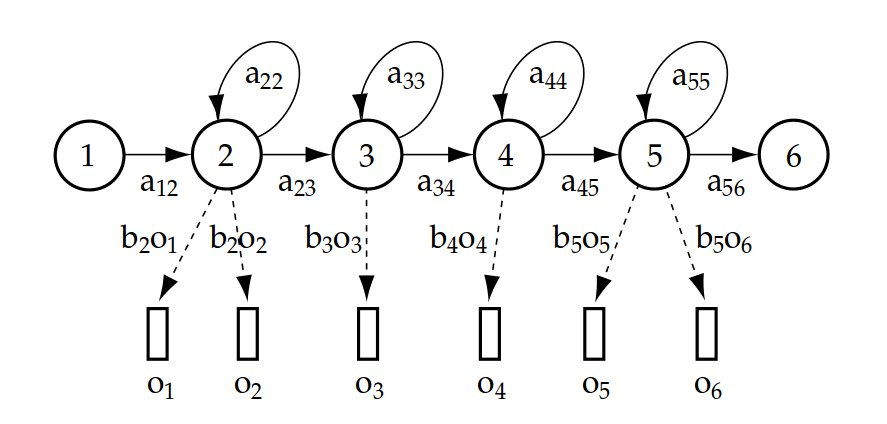
\includegraphics[width=0.7\textwidth]{images/hmm_structure.jpg}
\caption{6-state HMM structure. the states are denoted with numbered circles. State transitions probability form state $i$ to state $j$ are denoted by $a_{ij}$. Output probability densities of state $i$ are denoted $b_{i}$ and the observation generated at time instant $t$ is $o_{t}$}
\label{fig:hmm_structure}
\end{centering}
\end{figure}

Finding the probability that the observed sequence was produced by the given model causes the first problem, but it can be used to score different models based on how well they match the given observation sequence. This probability is calculated by the equation:

\begin{equation}
P(\mathbf{O}|\lambda) = \sum_{all \ Q} P(\mathbf{O}|\mathbf{Q},\lambda) \cdot P(\mathbf{Q}|\lambda)
\end{equation}

Although the calculation of $P(\mathbf{O}|\lambda)$ is straightforward, it involves on the order of $2 \cdot T \cdot N^{T}$ calculations, which is far from being efficient.
%
To reduce the computational cost of this calculation, this problem is usually evaluated with the Forward-Backward algorithm (see \cite{rabiner89}), requiring $N^{2} \cdot T $ calculations.

To solve the second problem we need to find the single best state sequence for a given observation sequence and a given model, i.e. we need to find $Q* = arg max_{Q} P(\mathbf{Q}|\mathbf{O},\lambda)$. 
%
This is usually solved using the Viterbi-algorithm \cite{viterbi67}. 

The third problem listed before is the most difficult one to solve.
%
Solving the model which maximizes the probability of the observation sequence has no known analytical solution. 
%
In stead, gradient based algorithms and iterative algorithms such as the Expectation-Maximization (EM) algorithm \cite{dempster77} are being used for maximizing $P(\mathbf{O}|\lambda)$.

HMMs have the possibility of being extended with various features, increasing the versatility and efficiency depending on the needs of the user. 
%
For example, state tying, state duration densities and inclusion of null transitions are among the extensions proposed.
%
More information about HMMs can be found in  \cite{rabiner89} and \cite{rabiner93}.

\subsection{HMM-Based Speech Synthesis System}
\label{hmm_synthesis_based_system}
In this project an HMM-based speaker-adaptive synthesis system will be used to synthesize speech with different speaker styles.
%
In \cite{tokuda13} a general overview of speech synthesis based in HMMs can be found.

\subsubsection{System Overview}
\label{hmm_synthesis_based_system_overview}
The general overview of a HMM-based synthesis system is ilustrated in Figure \ref{fig:hmm_system_overview}.

\begin{figure}[!htb]
\begin{centering}
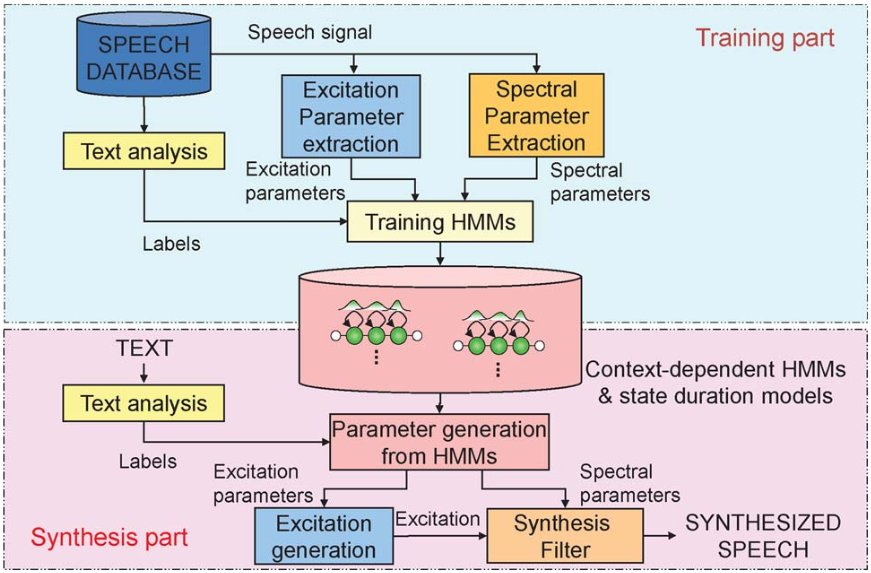
\includegraphics[width=\textwidth]{images/hmm_based_system_overview.jpg}
\caption{Overview of an HMM-based speech synthesis system \cite{tokuda13}}
\label{fig:hmm_system_overview}
\end{centering}
\end{figure}

An HMM-based system can be divided in two major parts: training and synthesis. 
%
In the training part, the vocoder extracts the speech parameters of every sample in the speech database and the labels containing the translation to the phonetic unit used, as explained in Section \ref{speech_synthesis_systems_tts}.
%
Then, the obtained parameters are modeled in the framework of the HMM.
%
The goal of the synthesis part is to produce a speech waveform according to the text input.
%
This process begins with the analysis of the text, as in the training part, in order to concatenate the required HMMs for that particular sentence and generate the parameters to feed the synthesis module and generate the speech waveform.

In this project we will be using a speaker-adaptive system. 
%
Thus, there is an extra part not represented in the general overview of an HMM-based system shown in Figure \ref{fig:hmm_system_overview}: adaptation. 
%
Before the parameter generation a transformation is applied to the context-dependent HMMs and the state duration models, aiming to convert them into models of the target speaker.
%
Adaptation makes synthesis with little data from a specific speaker possible, but it must be done from a good average voice model, built out from several speakers, and the differences between the average voice model and the target speaker will highly affect the similarity between the real speaker and the synthetic voice.
%
In Section \ref{hmm_synthesis_adaptation} an overview of a speaker-adaptive system is given and the adaptation technique used is explained.

The next sections explain the different steps that are done while constructing the HMM-based speech synthesis system.

\subsubsection{Speech Parametrization}
\label{hmm_synthesis_parametrization}
The first step of the training part is to extract from the speech signal a few parameters which function is to describe the essential characteristics of the speech signal as accurately as possible, compressing the original information.
%
A very efficient way was found in separating the speech signal to source and filter \cite{Fant1970}, both represented by coefficients. 
%
Both, STRAIGHT and GlottHMM follow the source-filter theory, although it is not the only approach to this problem, it is a functional trade-off between the accurate but complex direct physical modelling and a reasonable analytic solution.
%
This approach models the speech as a linear system where the ideal output is equivalent to the physical model, but the inner structure does not mimic the speech production physical structure.

In Section \ref{vocoders} the differences between the speech parametrization done by GlottHMM and STRAIGHT can be found, as they implement a different solution to this problem while following the same source-filter structure.

\subsubsection{Training of HMM}
\label{hmm_synthesis_training}
Once the parametrization is done, the speech features obtained are used to train a voice model. 
%
During the training, maximum-likelihood estimation of the HMM parameters is performed.

The case of speech synthesis is a particular one, as the $F_{0}$ values are not define in the unvoiced region, the observation sequence of $F_{0}$ is composed of 1-D continuous values and also discrete values or symbols representing the unvoiced.
%
HMMs need to model both the excitation and spectral parameters at the same time, but applying both the conventional discrete and continuous HMMs to model $F_{0}$ cannot be done directly. 
%
Thus, to model the $F_{0}$ observation sequence, HMM-based speech systems use multispace probability distributions \cite{tokuda2002multi}. 
%
Tipically, the multispace distribution consists of a continuous distribution for the voiced frames an a discrete one for the unvoiced. 
%
Switching according to the space label associated with each observation makes possible to model variable dimensional vector sequences, in our case, the $F_{0}$ observation sequence.
% 
To keep synchronization between the spectral and the excitation parameters, they are simultaneously modelled by separate streams in a multistream HMM, which uses different output probability distributions depending on the features.

As shown in Figure \ref{fig:hmm_system_overview}, the training takes into account the duration and context to model the different HMMs.
%
The duration modelling specifies for each HMM a state-duration probability distribution that are used to model the temporal structure of the speech in detriment of transition probabilities.

The context dependency of the HMMs is needed in speech synthesis to deal with the linguistic specifications.
%
Different linguistics contexts, such as tone, pitch accent or speech stress among others, are used by HMM-based speech synthesis to build the HMMs.
%
Spectral parameters are mainly affected by phoneme information, but prosodic and duration parameters are also affected by linguistic information. In \cite{tokuda13} some of the contexts used in English can be found.

Finally, it is important to note that there are too many contextual factors in relation with the amount of the speech data available. 
%
Increasing the speech data will increase the number of contextual factors and exponentially their combinations.
%
Hence, limited amount of data will limit the accuracy and robustness of the HMMs estimation.
%
To overcome this issue, tying techniques as state clustering and tying model parameters among several HMMs are used in order to obtain a more robust model parameters estimation.
%
It must be noticed that spectral, excitation and duration parameters are clustered separately as they have different context dependency.

Once the HMMs are estimated regarding the considerations explained, the training part is finished and a model is built.
%
If the model aims to reproduce one speaker, we would be talking about a speaker-dependent model.
%
However, a speaker-adaptive system as the one used in this project aims to synthesize different speakers from one model as starting point.
%
This model is called speaker-independent model, and the only difference with the speaker-dependent model so far in the HMM-based system construction is that the speech data is composed by several speakers to cover different speaker styles.
%
However, when using speaker-independent models aiming to adapt to different speakers, a technique called speaker-adaptive training (SAT) is used to generate an average voice model by normalizing interspeaker acoustic variation \cite{anastasakos1996, yamagishi2003training}.

\subsubsection{Adaptation}
\label{hmm_synthesis_adaptation}
Figure \ref{fig:hmm_system_overview} shows the overview of a general HMM-based speech synthesis system.
%
In order to build a speaker-adaptive system, there is a third part that must be added to the structure before the synthesis: adaptation.

As commented previously, HMM-based systems are quite flexible, resulting in a good quality adaptive systems.
%
Figure \ref{fig:hmm_system_adapt_overview} illustrates a HMM-based speaker-adaptive system, hence, it shows the basic structure of both systems compared in this project.

\begin{figure}[!htb]
\begin{centering}
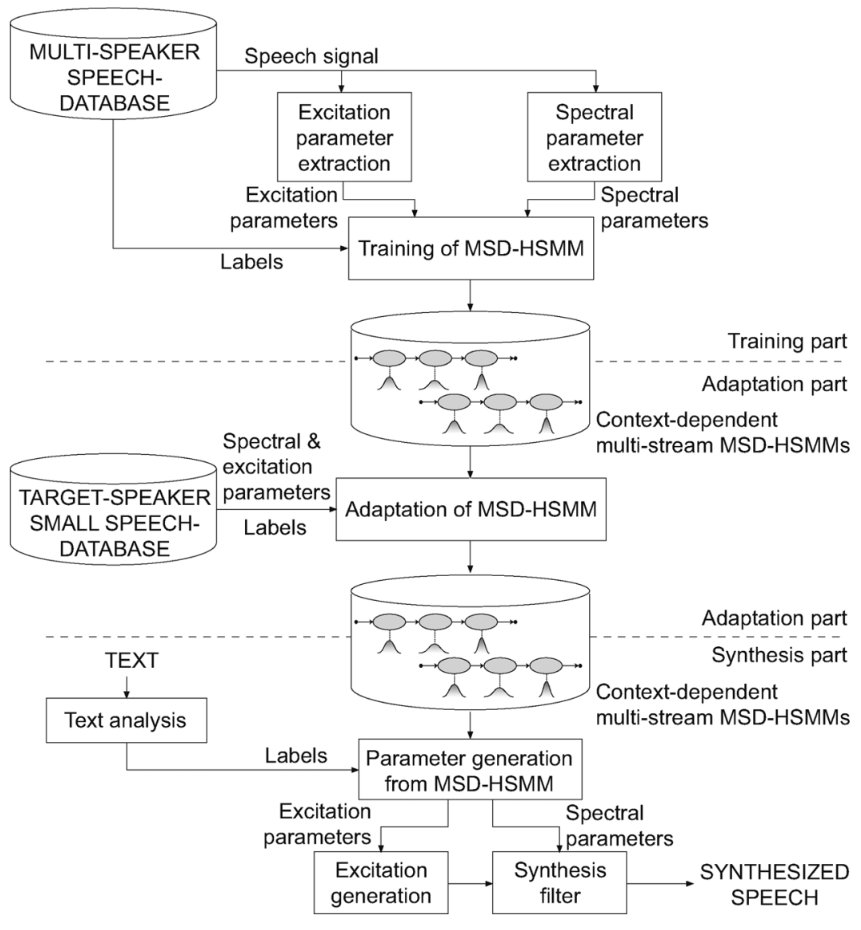
\includegraphics[width=0.8\textwidth]{images/hmm_based_system_adapt_overview.jpg}
\caption{Overview of an HMM-based speaker-adaptive speech synthesis system \cite{yamagishi2009}}
\label{fig:hmm_system_adapt_overview}
\end{centering}
\end{figure}

The adaptation layer between the training and the synthesis part is the only difference between the structures of an adaptive and a non-adaptive system.
%

Many adaptation techniques are used in HMM-based speaker-adaptive systems, all of them targeting the same: transforming an average voice model to match a predefined target using a very small amount of speech data.
%
Among the different targets we can find for example speaker adaptation or expressive speech.
%
In \cite{tokuda13} we can find several issues where adaptation techniques are helpful. 

Within the speaker-adaptive challenge, several techniques to approach a satisfying solution are available. 
%
\cite{yamagishi2009} proposes an adaptation algorithm called constrained structural maximum a posterior lineal regression (CSMAPLR) and compares several adaptation algorithms to figure out which one to use in which conditions.

The adaptations made during this project and in \cite{karhila_jstsp_14} use the CSMAPLR algorithm.
%
This algorithm combines different adaptation algorithms in a defined order. The algorithms used are:

\begin{itemize}
	\item Constrained maximum-likelihood liner regression (CMLLR)
	\item Maximum a posteriori (MAP)
	\item Structural maximum a posterior (SMAP)
\end{itemize}

When adapting in speech synthesis, it is important to adapt both the mean vectors and covariance matrices of the output and duration probability density functions, as the covariance is also an important factor affecting synthetic speech.
%
This is the reason to use CMLLR in stead of the unconstrained version.

The CMLLR adaptation algorithm uses the maximum-likelihood criterion \cite{digalakis1995speaker, gales1998maximum} to estimate the transforms. 
%
The criterion works well when large amount of data is available.
%
However, in the adaptation stage the amount of data is limited, a more robust criterion must be found: MAP.
%
The basis of MAP algorithm are explained in \cite{gauvain1994maximum} and an overview is given in \cite{yamagishi2009}.

In SMAP \cite{shinoda2001structural} the tree structures of the distributions effectively cope with the control of the hyperparameters.

\subsubsection{Synthesis}
\label{hmm_synthesis_synthesis}
The lower part of Figures \ref{fig:hmm_system_overview} and \ref{fig:hmm_system_adapt_overview} show the synthesis part of an HMM-based speech synthesis system.
%
The first step is to convert the given text into a sequence of context dependent labels.
%
Then, context-dependent HMMs are concatenated according to the labels calculated in the previous step, determining the duration of each state to maximize its probability based on its state duration probability distribution.
%
Once the original sentence has been translated to context-dependent HMMs, a sequence of speech parameters is generated and using both the spectral and excitation parameters the speech waveform is produced by the correspondent vocoder. 